\documentclass{article}

% Language setting
% Replace `english' with e.g. `spanish' to change the document language
\usepackage[english]{babel}

% Set page size and margins
% Replace `letterpaper' with `a4paper' for UK/EU standard size
\usepackage[a4paper,top=2cm,bottom=2cm,left=3cm,right=3cm,marginparwidth=1.75cm]{geometry}

% Useful packages
\usepackage{amsmath}
\usepackage{graphicx}
\usepackage[colorlinks=true, allcolors=blue]{hyperref}

\title{TDT4171 — Artificial Intelligence Methods \\ Assignment 8 - Deep Learning}
\author{Erik Storås Sommer - 535006}
\date{March 2023}

\begin{document}
\maketitle
\setlength{\parindent}{0pt}

\section*{Exercise - FNN and RNN with Keras}

In this assignment, the objective was to implement and train feedforward and recurrent neural networks using Keras.
Several different architectures and hyperparameters were tested to evaluate their performance.
This report presents the results from theise decisions.

\subsection*{Hyperparameters}

The hyperparameters used for the two neural networks are presented in figure \ref{fig:image1}. I found little to no difference in accuracy when adding more than 2 hidden layers.
The activation function used for the hidden layers is relu, since it is the most common activation function for hidden layers and switching to others did not make a big difference in accuracy.
The activation function for the LSTM layer is sigmoid and the recurrent activation function is tanh.
The default values for these two parameters are the oposite, but I found better results switching them.
Forthermore, since the target for the dataset is either 0 or 1, the output layer has only one neuron using the sigmoid activation function.
The loss function used is binary crossentropy, and the optimizer is adam.
All are suitable for this type of problem.
Additionally, the average length of the training data was utilized to set the maxlen parameter, which is used to pad the training and test data to a uniform length.

\begin{figure}[hbtp]
    \centering
    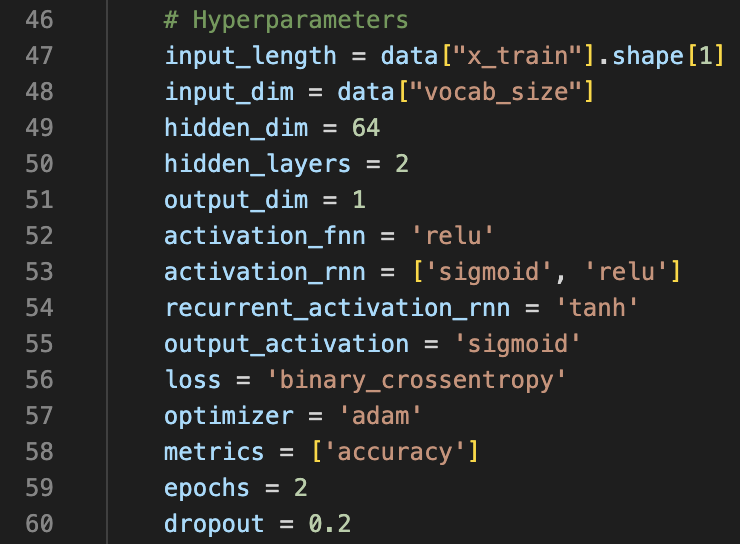
\includegraphics[width=0.85\textwidth]{hyperparameters.png}
    \caption{Hyperparameters used for the neural networks}
    \label{fig:image1}
\end{figure}

\newpage

\subsection*{Results}

By using the parameters in figure \ref{fig:image1}, the model was able to achieve a test accuracy of above 90\% on both the feedforward and recurrent neural network.
The time it took to train the feedforward model was greatly lower than the recurrent model, but the recurrent model was able to achieve a higher accuracy.
This is due to the fact that the recurrent model uses previous input to make a more educated prediction, while the feedforward model is only able to use the current input.
The results are presented in figure \ref{fig:image2}.

\begin{figure}[hbtp]
    \centering
    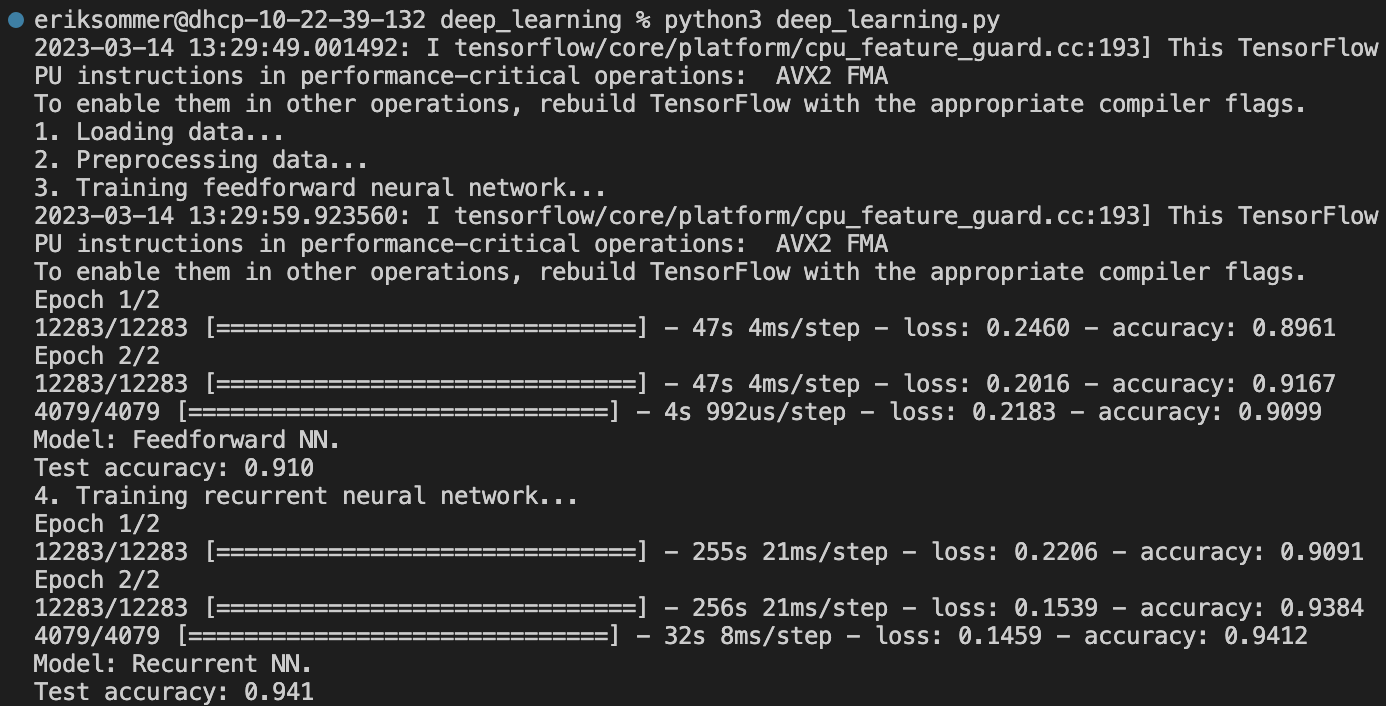
\includegraphics[width=\linewidth]{output.png}
    \caption{Output from running the attached python file}
    \label{fig:image2}
\end{figure}

\end{document}